\lesson{Torque}
The \textit{change in rotational motion} depends on both the \textit{force applied} and 
\textit{location} that this force was applied from. The measure of this change in rotational motion
is measured by the quantity \textbf{torque}, denoted by $\vect{\tau}$. Torque is defined to be
\[
    \vect{\tau}=\vect{r}\times\vect{F}
\]
And by definition of cross product, the magnitude of the torque is
\[
    \tau=rFsin\theta=Fd
\]
Where $d$ is the perpendicular distance from the orientation axis to the line of action of 
$\vect{F}$, called the \textbf{moment arm} (or \textit{lever arm}) of $\vect{F}$. See Figure 
\ref{fig:torque}.

\begin{figure}[ht!]
    \centering
    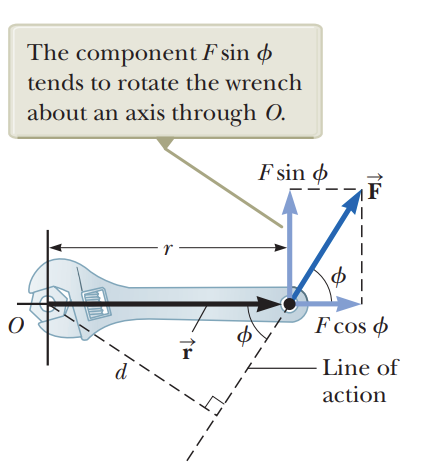
\includegraphics[width=0.4 \textwidth]{../figures/torque.png}
    \caption{}
    \label{fig:torque}
\end{figure}

\subsection{Rigid Object Under a Net Torque and Moment of Inertia}
For a particle with mass $m$ rotating in a circle of radius $r$
\[
    \Sigma F_t=ma_t
\]
The net torque is
\[
    \Sigma\tau=\Sigma F_tr=(ma_t)r
\]
But recalling that $a_t=r\alpha$
\begin{align*}
    \Sigma\tau&=(mr\alpha)r\\
    &=(mr^2)\alpha\\
    \Sigma\tau&=I\alpha
\end{align*}
Where we let $I=mr^2$. The quantity $I$ is called the \textbf{moment of inertia}. For a given rigid
body that is made up of a collection of particles, even though they may have different translational
accelerations $a_i$, they all have the \textit{same} angular acceleration $\alpha$. Therefore
\begin{align*}
    \Sigma \tau_\text{ext}&=\Sigma_i\tau_i\\
    &=\Sigma_im_ir_i^2\alpha\\
    &=(\Sigma_im_ir_i^2)\alpha\\
    &=I\alpha
\end{align*}
Where
\[
    I=\Sigma_im_ir_i^2
\]
Notice that this equation has the same form as Newton's second law for a system of particles
\[
    \Sigma\vect{F}_\text{ext}=M\vect{a}_\text{CM}
\]
Consequently, the moment of inertia $I$ must lay the same role in rotational motion as the role
that mass plays in translational motion: the moment of inertia is the resistance to changes in
rotational motion. See Figure \ref{fig:moments-of-inertia}.

\begin{figure}[ht!]
    \centering
    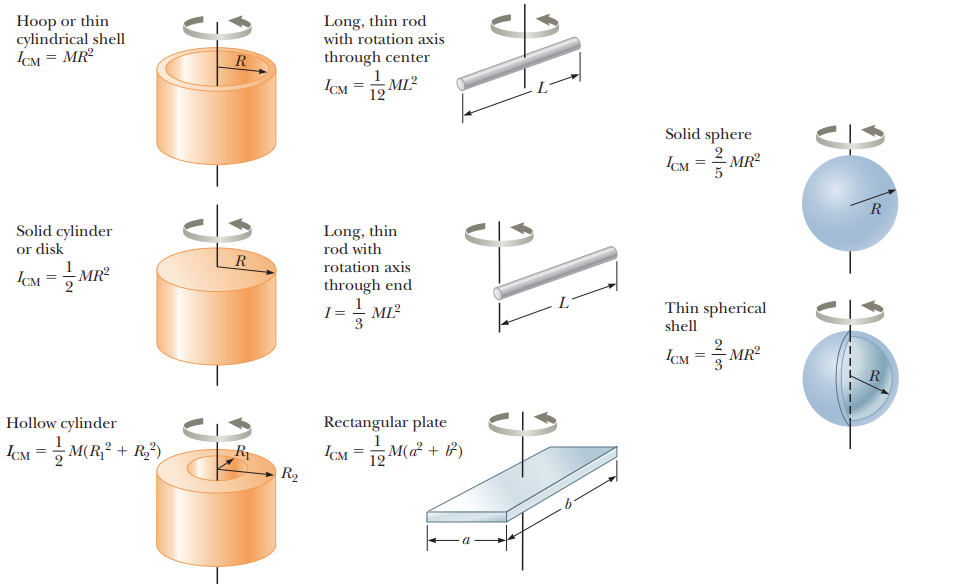
\includegraphics[width= \textwidth]{../figures/moments of inertia.png}
    \caption{Moments of inertia of homogeneous rigid objects with different geometries}
    \label{fig:moments-of-inertia}
\end{figure}

\subsection{Deriving Moments of Inertia for Geometries}
Because the moment of inertia for a rigid body is defined to be
\[
    I=\Sigma_im_ir_i^2
\]
If we were to consider for an infinitesimal number of particles that make up that rigid body, the
summation simplifies to become
\[
    I=\int r^2\,dm
\]

\subsection{Deriving Moment of Inertia Formula for Uniform Thin Rod with Axis Through the Center}
Suppose we had a rod that was oriented along the x-axis and it were to be rotated about the z-axis
(Figure \ref{fig:rod-moment-of-inertia}). 
\begin{figure}[ht!]
    \centering
    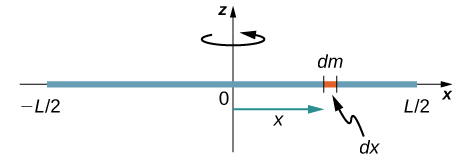
\includegraphics[width=0.4 \textwidth]{../figures/rod moment of inertia.png}
    \caption{}
    \label{fig:rod-moment-of-inertia}
\end{figure}
But since $I=\int r^2dm$ and it is impractical to integrate over mass, we will perform u-substition.
We will do this using the linear mass density $\lambda$ of the object, which is the mass per unit
length. Since the mass density of this object is uniform
\begin{align*}
    \lambda&= \frac{m}{x}\\
    m&=\lambda x\\
    dm&=d(\lambda x)\\
    &=\lambda dx
\end{align*}
So performing this substitution yields
\begin{align*}
    I&=\int x^2\,dm\\
    &=\int x^2\lambda\,dx\\
    &=\lambda\int x^2\,dx
\end{align*}
For the limits of integration, we are integrating from $x=-\frac{L}{2}$ to $x=\frac{L}{2}$
\begin{align*}
    I&=\lambda\int_{-\frac{L}{2}}^{\frac{L}{2}}x^2\,dx\\
    &=\lambda \left[\frac{1}{3}x^3\right]_{-\frac{L}{2}}^{\frac{L}{2}}\\
    &=\frac{\lambda}{3}\left[\frac{L^3}{8}+\frac{L^3}{8}\right]\\
    &=\frac{1}{12}\lambda L^3
\end{align*}
But noting that $\lambda=\frac{M}{L}$ yields the final equation
\[
    I=\frac{1}{12}ML^2
\]

\subsection{Deriving Moment of Inertia for a Uniform Thin Rod with Axis at the End}
This is a simple setup which has the moment of inertia evaluating to one simple integral
\begin{align*}
    I&=\lambda\int_0^Lx^2dx\\
    &=\lambda \left[\frac{1}{3}x^3\right]_0^L\\
    &=\frac{1}{3}\lambda L^3\\
    &=\frac{1}{3}ML^2
\end{align*}

\subsection{Deriving Moment of Inertia for a Disk Through the Center}
We can utilize the disk method for integration (Figure \ref{fig:disk-moment-of-inertia}).
\begin{figure}[ht!]
    \centering
    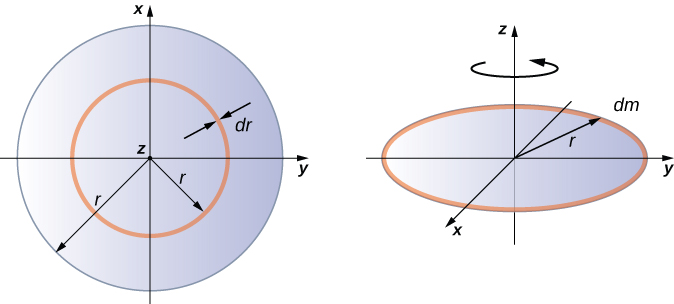
\includegraphics[width=0.8 \textwidth]{../figures/disk moment of inertia.jpg}
    \caption{}
    \label{fig:disk-moment-of-inertia}
\end{figure}
We start with the relationship for the surface mass density, which is the mass per unit surface
area. Since it is uniform, the surface mass density $\sigma$ is constant
\begin{align*}
    \sigma&=\frac{m}{A}\\
    m&=\sigma A\\
   dm&=\sigma(dA)
\end{align*}
Since we have the relationship $A=\pi r^2$, we can calculate for $dA$
\begin{align*}
    dA&=d(\pi r^2)\\
    &=2\pi rdr
\end{align*}
So integrating from $r=0$ to $r=R$ yields
\begin{align*}
    I&=\int_0^Rr^2[\sigma(2\pi r)]\,dr\\
    &=2\pi\sigma\int_0^R r^3\,dr\\
    &=2\pi\sigma \left[\frac{1}{4}r^4\right]_0^R\\
    &=\frac{\pi\sigma}{2}R^4
\end{align*}
But rectall that $\sigma=\frac{m}{A}=\frac{m}{\pi R^2}$ so
\begin{align*}
    I&=\frac{m}{\pi R^2}\frac{\pi}{2}R^4\\
    &=\frac{1}{2}mR^2
\end{align*}

\subsection{Parallel-Axis Theorem}
The similarity between the process of finding the moment of inertia of a rod about an axis through
its middle and about an axis through its end is striking, and suggests that there might be a simpler
method for determining the moment of inertia for a rod about any axis parallel to the axis through
the center of mass. Such an axis is called a \textbf{parallel axis}, and the \textbf{parallel-axis
theorem} is stated as
\[
    I_\text{parallel-axis}=I_\text{center of mass}+md^2
\]
Where $m$ is the mass of an object and $d$ is the distance from an axis through the object's 
center of mass to a new axis.

\subsection{Derivation of Parallel-Axis Theorem}
We may assume, without loss of generality, that in a Cartesian coordinate system the distance
between the axes lies along the x-axis and that the center of mass lies at the origin (Figure
\ref{fig:parallel-axis-theorem}). The moment of inertia relative to the z-axis is then
\[
    I_\text{CM}=\int(x^2+y^2)\,dm
\]
\begin{figure}[ht!]
    \centering
    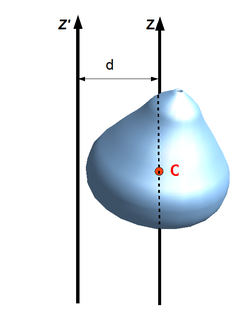
\includegraphics[width=0.3 \textwidth]{../figures/parallel axis theorem.png}
    \caption{}
    \label{fig:parallel-axis-theorem}
\end{figure}
The moment of inertia relative to the axis $z'$, which is at a distance $D$ from the center of
mass along the x-axis, is
\[
    I=\int((x-D)^2+y^2)\,dm
\]
Expanding the bracket yields
\[
    I=\int(x^2+y^2)\,dm+D^2\int dm-2D\int x\,dm
\]
And notice that the first term is $I_\text{CM}$, the second term becomes $MD^2$, while the
third term is a multiple of the x-coordinate of the center of mass which is $0$ since the center of
mass lies at the origin. So the equation becomes
\[
    I=I_\text{CM}+MD^2
\]